\documentclass{article}
\usepackage[spanish]{babel}
\usepackage{hyperref}
\usepackage{graphicx}
\usepackage{float}
\graphicspath{ {./images/} }
\hypersetup{
	colorlinks,
	citecolor=black,
	filecolor=black,
	linkcolor=black,
	urlcolor=black
}

\title{Visor arroz - Manual de usuario}

\begin{document}

\maketitle

\begin{center}
	
\includegraphics[width=0.2\textwidth]{andalucia.jpg}
	\hspace{1cm}
	\centering
	
\includegraphics[width=0.14\textwidth]{Logo_UCO.png}
	\hspace{1cm}
	\centering
	
\includegraphics[width=0.27\textwidth]{etsiam.jpg}
\end{center}

\newpage

\tableofcontents

\listoffigures

\newpage

\section{Requisitos}

Para la ejecución del visor, es necesario tener instalado un navegador web. Los navegadores web que pueden utilizarse junto con las versiones que se han probado son los siguientes:

\begin{itemize}
	\item Firefox 75.0
	\item Chrome 81.0.4044.138
	\item Opera 68.0.3618.63
\end{itemize}

\section{Abrir Visor arroz}

Para abrir el visor, podemos hacerlo de dos formas. Bien abriendo directamente el fichero 'html' con el navegador correspondiente, o bien arrastrando el fichero 'html' al navegador. 

\begin{figure}[H]
	\centering
	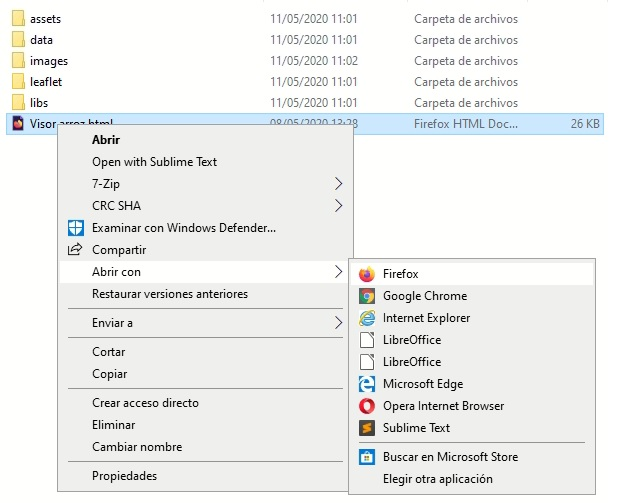
\includegraphics[width=0.8\linewidth]{image1.jpg}
	\caption{Abriendo el navegador desde el fichero}
	\label{fig:image1}
\end{figure}

\begin{figure}[H]
	\centering
	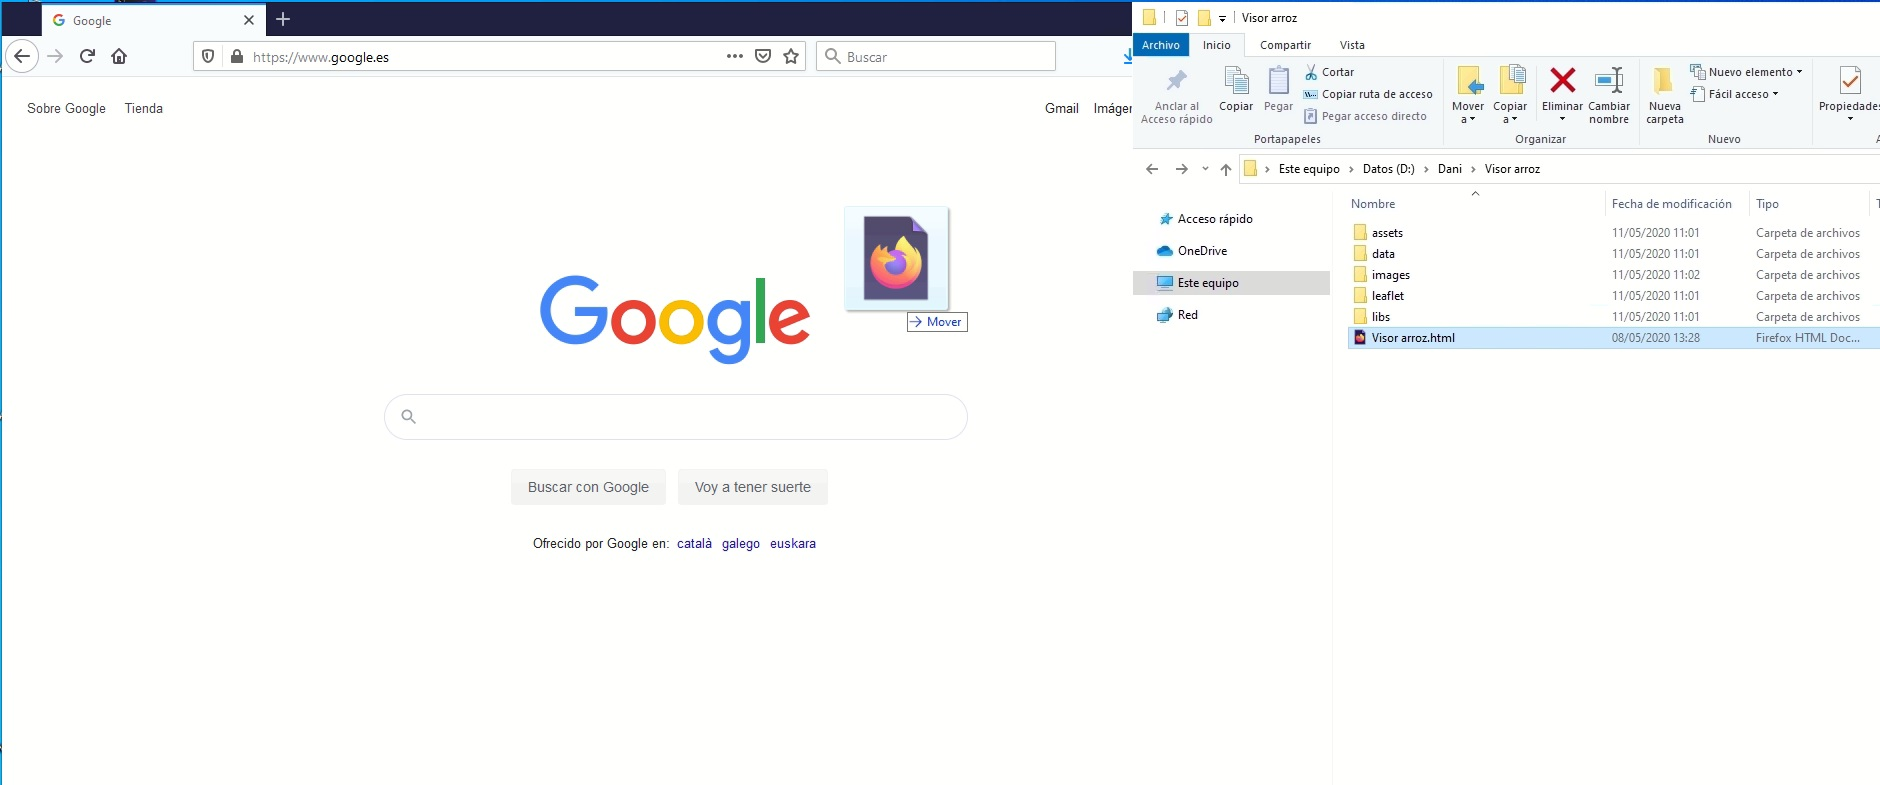
\includegraphics[width=0.8\linewidth]{image2.jpg}
	\caption{Abriendo el visor arrastrándolo al navegador}
	\label{fig:image2}
\end{figure}

De ambas formas, se nos abrirá correctamente el visor en el navegador que estemos utilizando.

\begin{figure}[H]
	\centering
	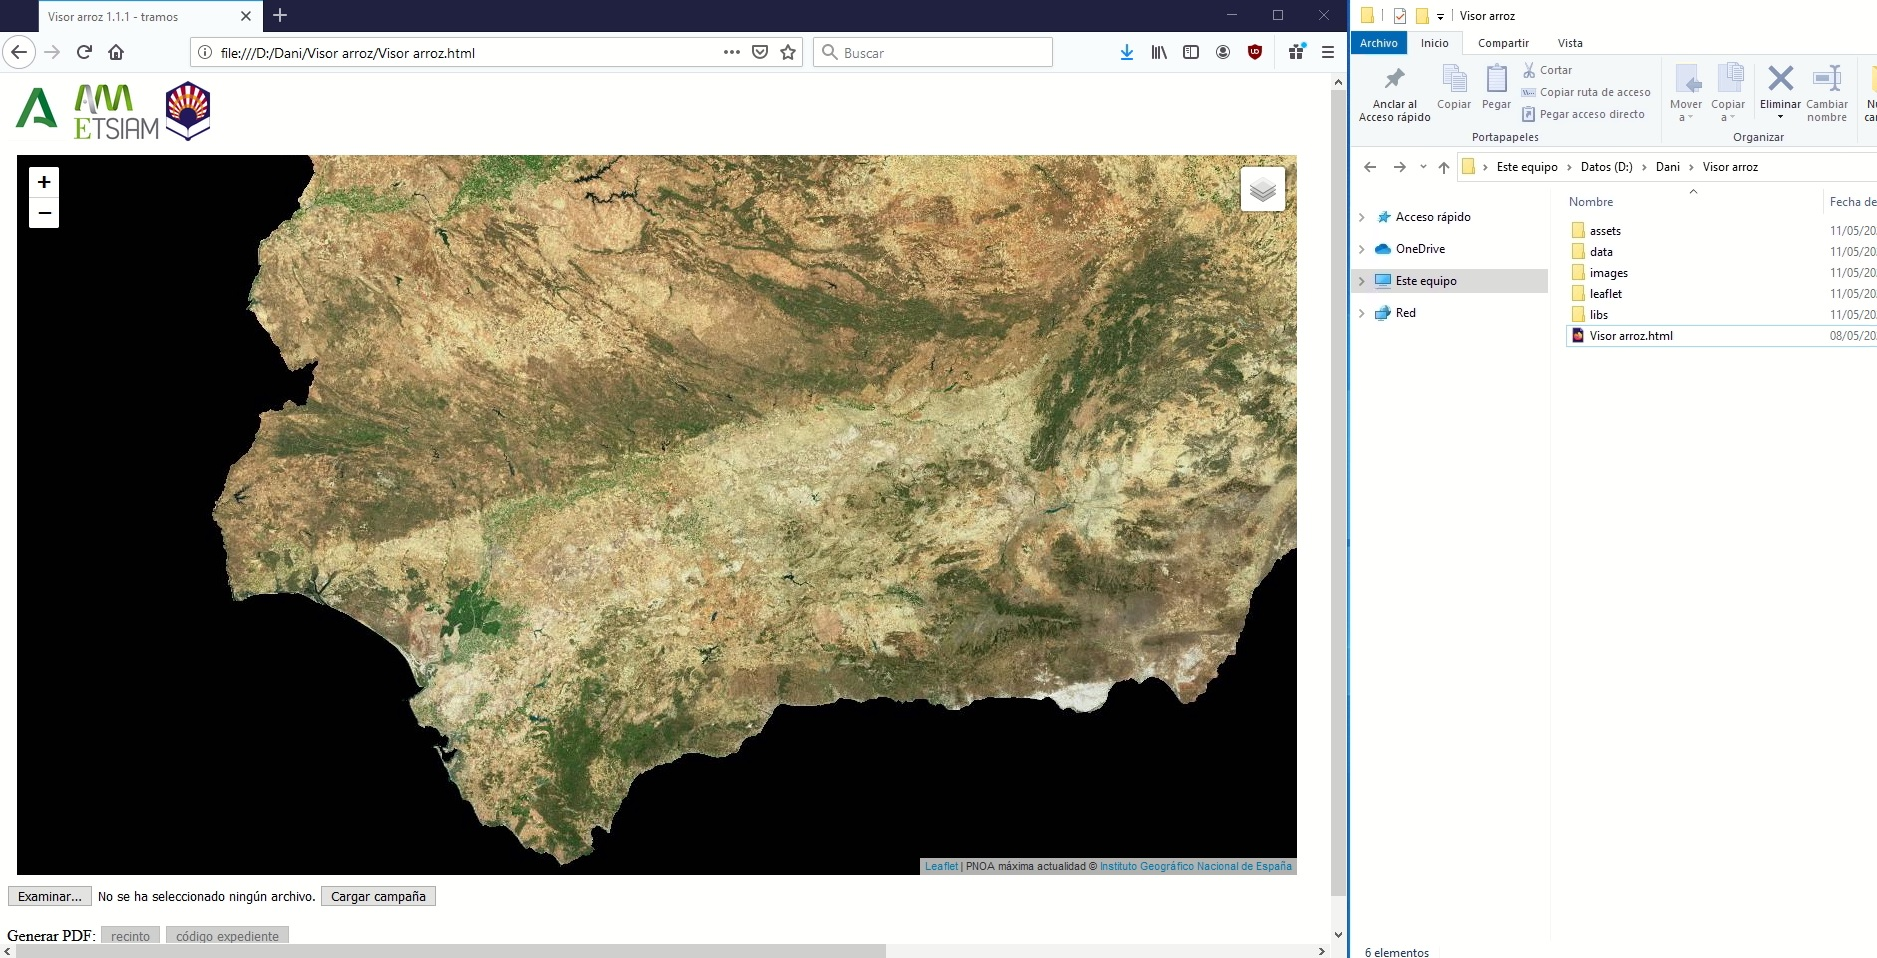
\includegraphics[width=0.8\linewidth]{image3.jpg}
	\caption{Visor abierto}
	\label{fig:image3}
\end{figure}

\newpage

\section{Descripción de la interfaz}

A continuación se explicará cada una de las opciones que componen el visor.

\begin{figure}[H]
	\centering
	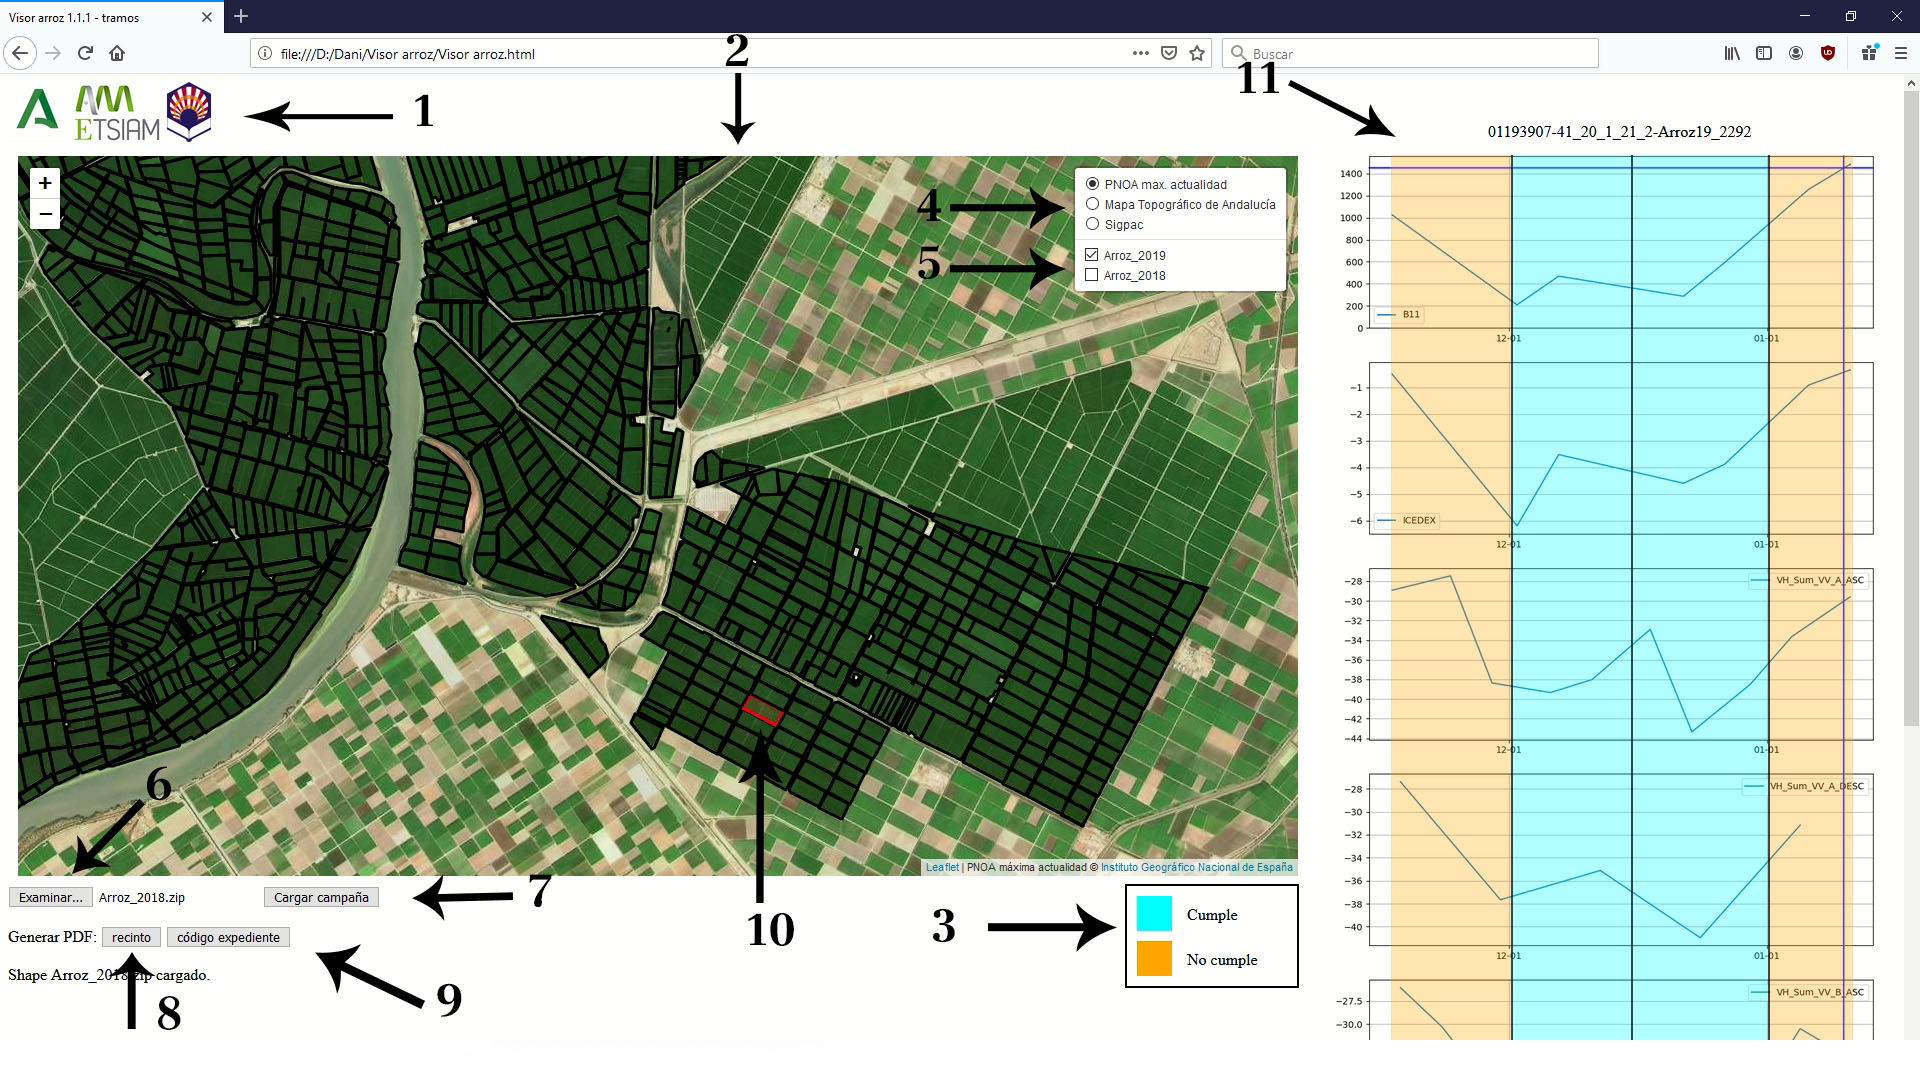
\includegraphics[width=0.8\linewidth]{image_interface.jpg}
	\caption{Interfaz visor}
	\label{fig:image-interfaz}
\end{figure}

\begin{enumerate}
	\item Logos con enlaces
	\item Visualización del mapa
	\item Leyenda
	\item Imágenes de satélite
	\item Mostrar campaña
	\item Buscar campaña
	\item Cargar campaña
	\item Guardar recinto
	\item Guardar recintos por código expediente
	\item Recinto seleccionado
	\item Series temporales de los índices
\end{enumerate}

\newpage

\subsection{Logos con enlaces}

Logos que contienen enlaces a sus correspondientes páginas web.

\subsection{Visualización del mapa}

Visor del mapa dónde se localizan los recintos y las diferentes geometrías.

\subsection{Leyenda}

Leyenda dónde se encuentran los colores correspondientes a los estados 'Cumple' y 'No cumple' de un recinto de arroz en la serie temporal.

\subsection{Imágenes de satélite}

'RadioButton' que permite cambiar las imágenes de satélite para la visualización del mapa.

\subsection{Mostrar campaña}

'CheckBox' que permite mostrar u ocultar en el mapa, las diferentes campañas que se han cargado previamente.

\subsection{Buscar campaña}

Botón que permite seleccionar la campaña a cargar.

\subsection{Cargar campaña}

Botón que permite cargar la campaña que se ha seleccionado previamente.

\subsection{Guardar recinto}

Botón que permite guardar en un fichero 'PDF' el recinto seleccionado en el mapa, junto con las series temporales, código de recinto, y una fotografía de la localización del recinto.

\subsection{Guardar recintos por código expediente}

Botón que permite hacer la misma acción que 'Guardar recinto', pero guardando solo aquellos recintos cuyo código expediente sea idéntico.

\subsection{Recinto seleccionado}

Región coloreada en rojo que marca el recinto que el usuario ha seleccionado en el mapa.

\subsection{Series temporales de los índices}

Series temporales de los diferentes índices marcando en colores, la salida de la red neuronal por cada quincena. Dichas series temporales corresponden al recinto que el usuario ha seleccionado en el mapa del visor (recinto coloreado en rojo).

\section{Pasos para cargar una campaña}

Una vez tengamos abierto el visor, lo primero que debe hacerse es cargar una campaña. Para ello, pinchamos en el botón 'Examinar...'

\begin{figure}[H]
	\centering
	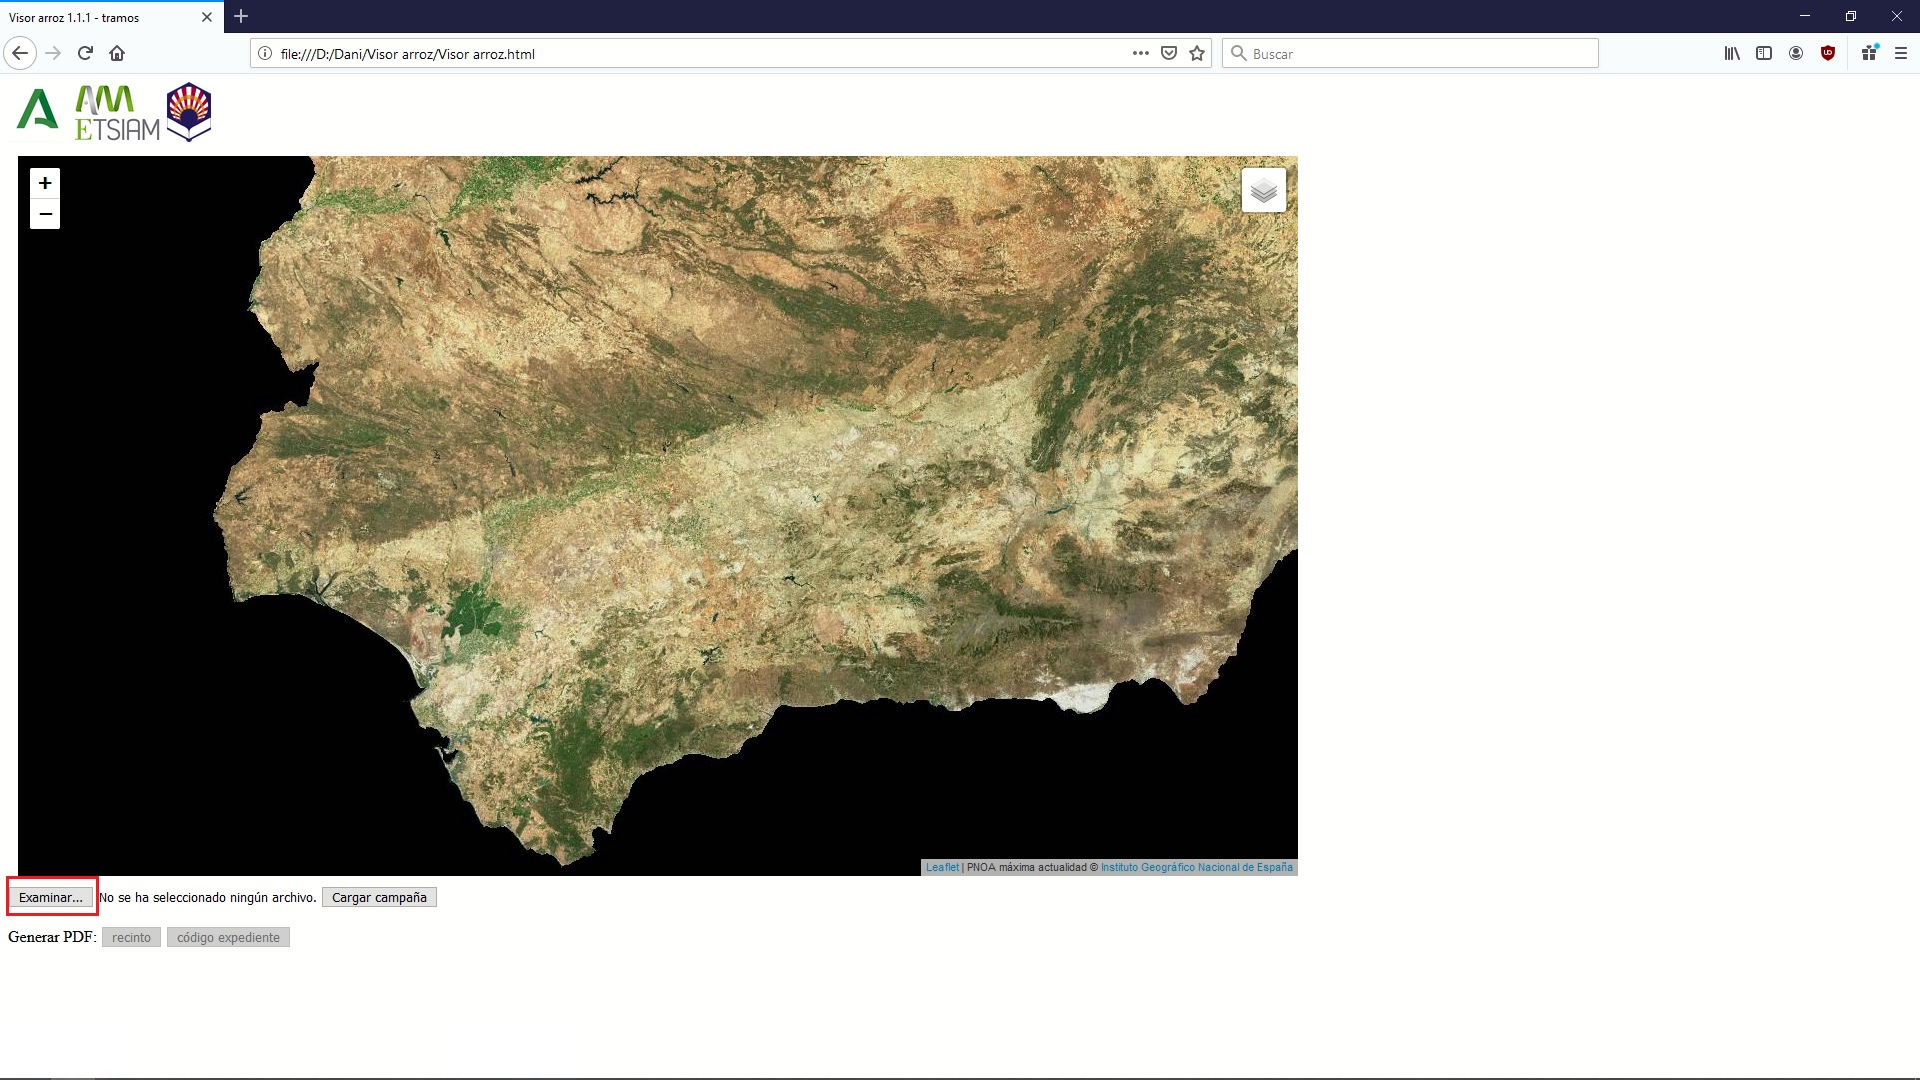
\includegraphics[width=0.8\linewidth]{examinar.jpg}
	\caption{Botón 'Examinar...'}
	\label{fig:examinar}
\end{figure}

Buscamos en la carpeta 'data'

\begin{figure}[H]
	\centering
	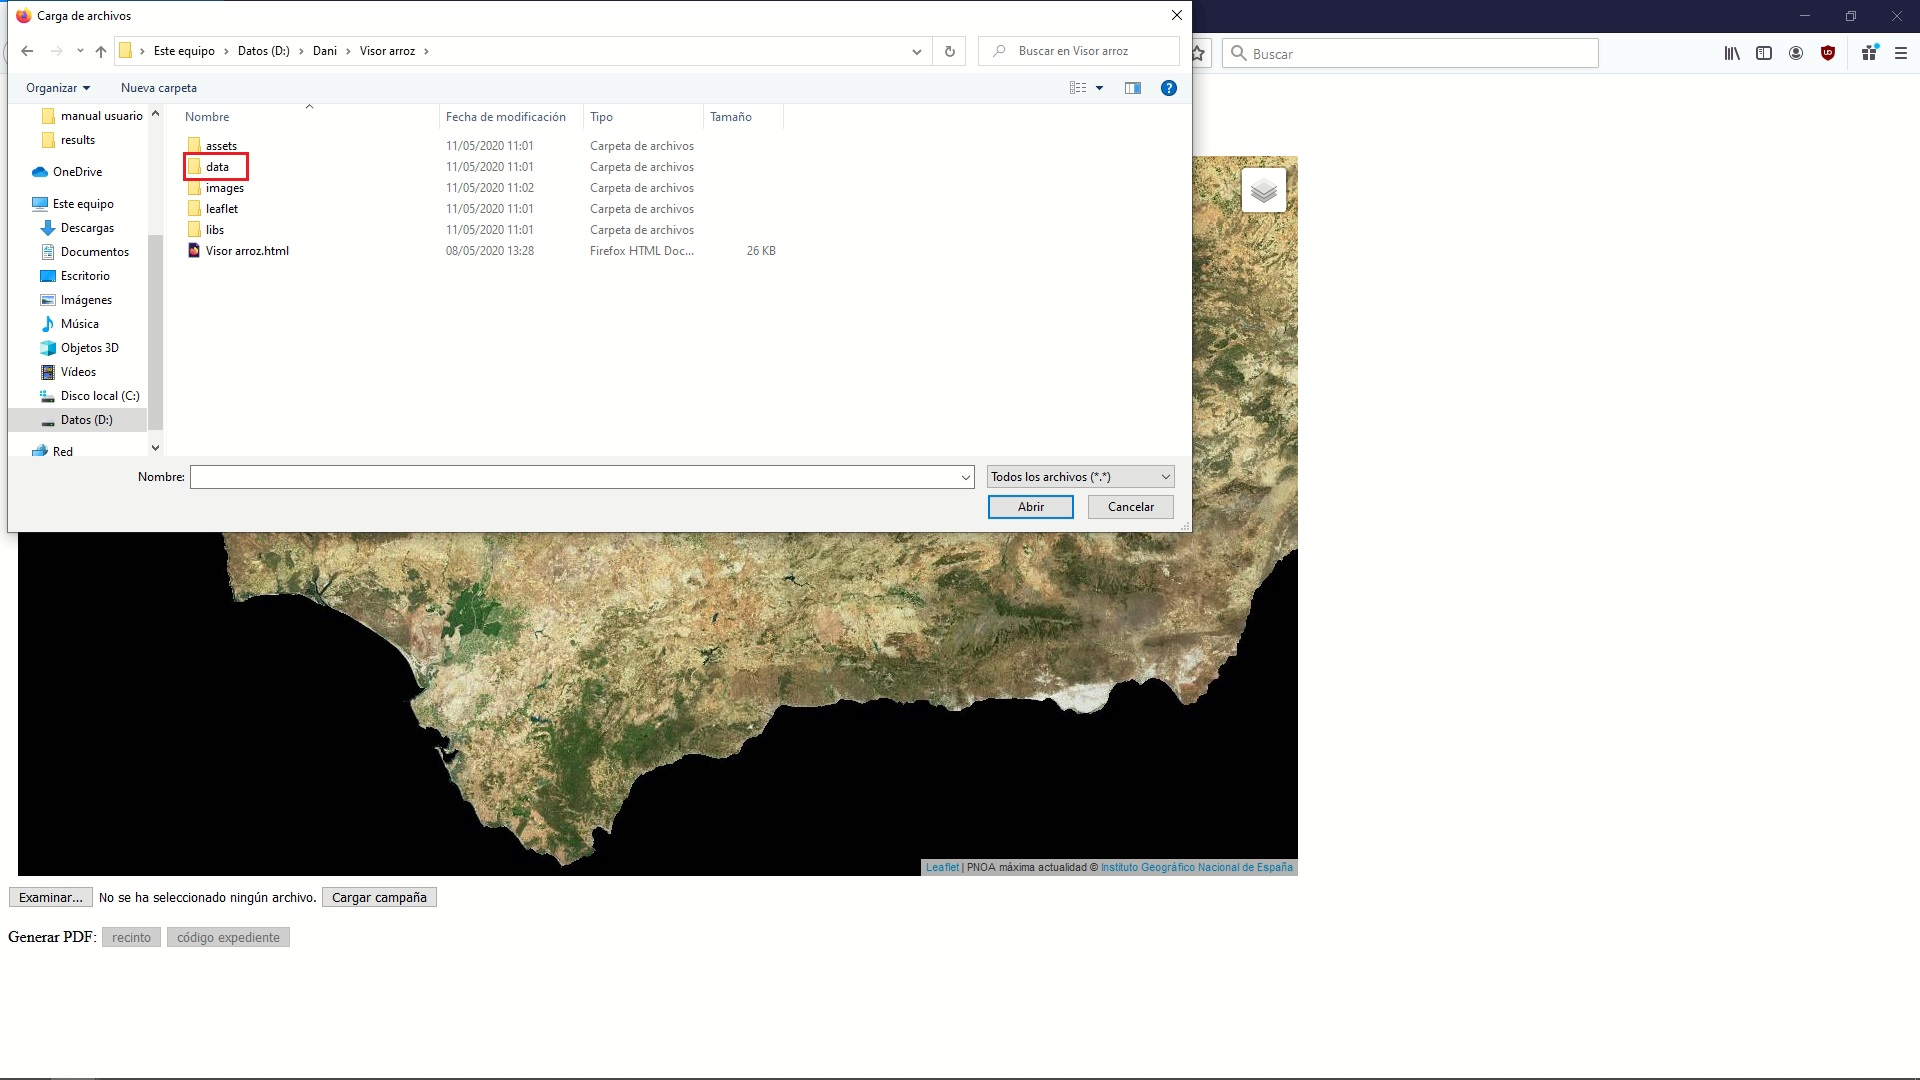
\includegraphics[width=0.8\linewidth]{data.jpg}
	\caption{Buscando carpeta data}
	\label{fig:data}
\end{figure}


Y finalmente seleccionamos la campaña que queramos utilizar.

\begin{figure}[H]
	\centering
	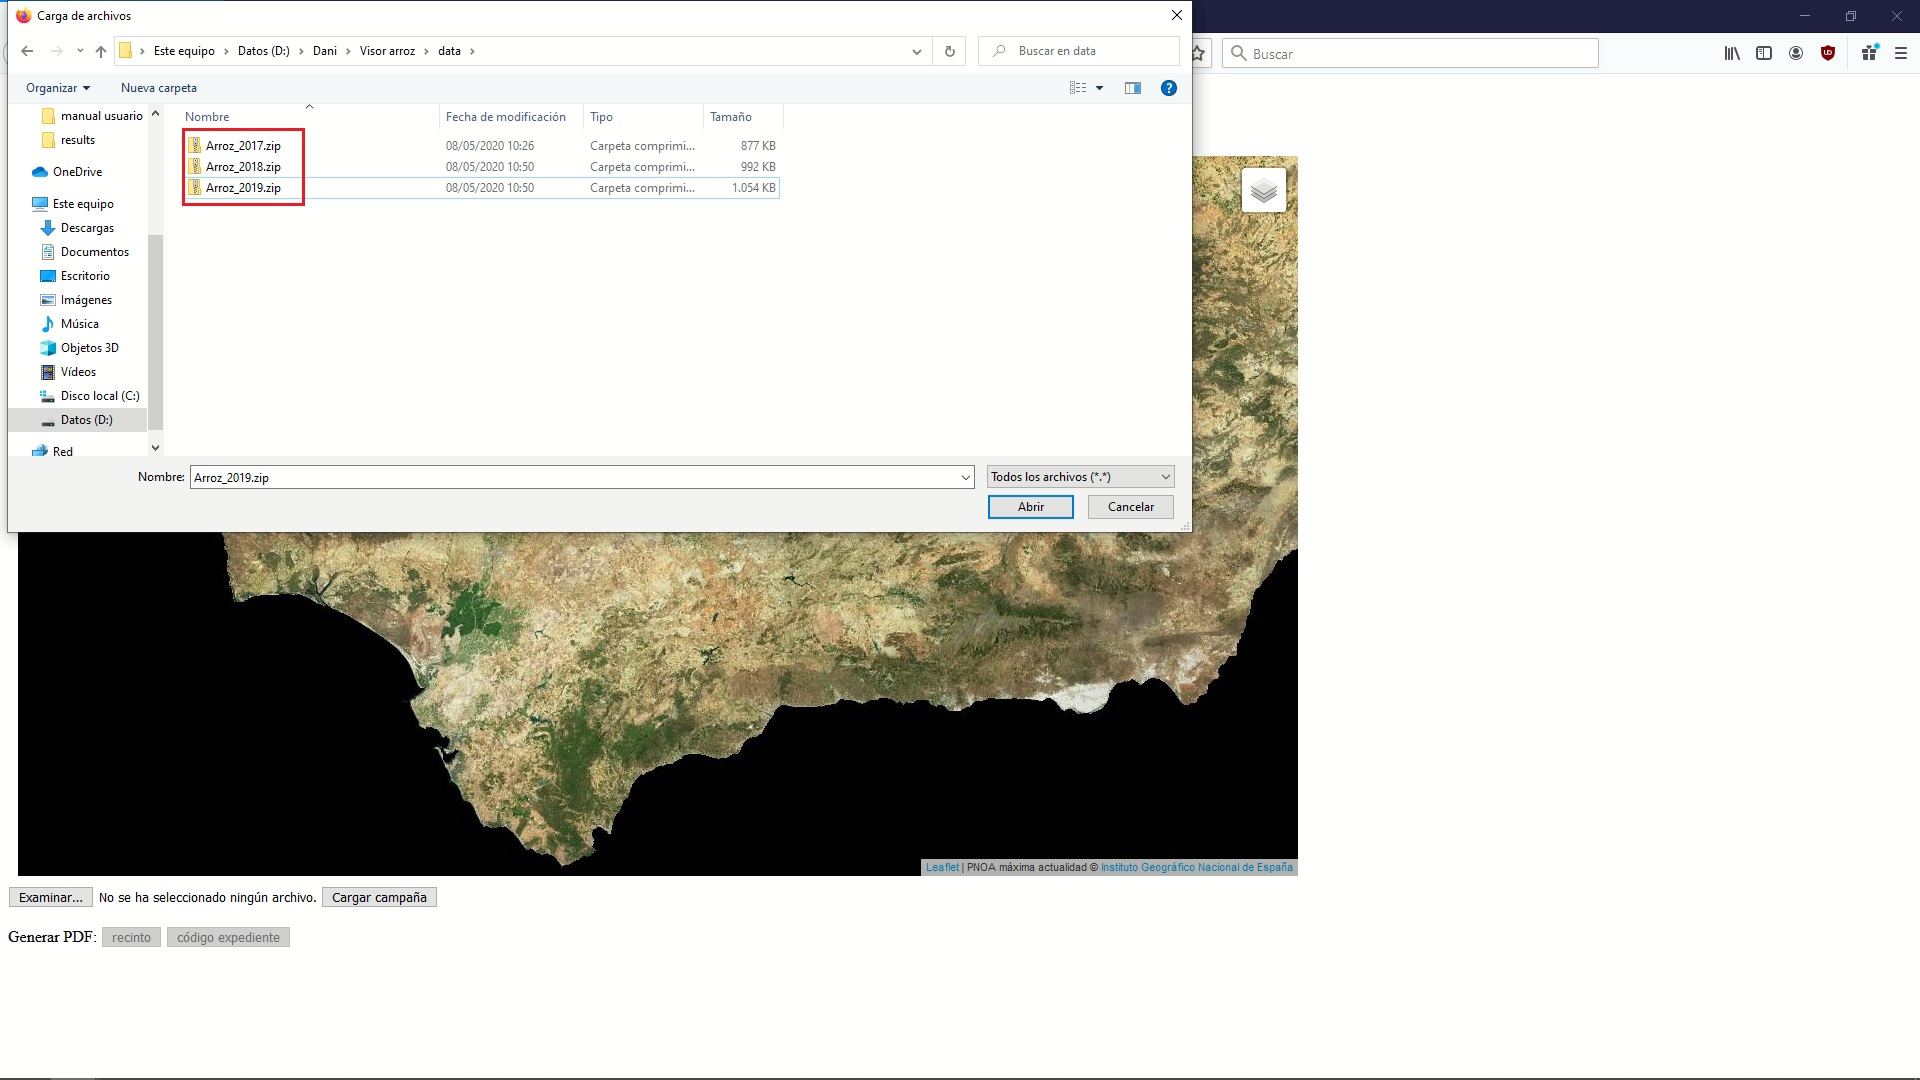
\includegraphics[width=0.8\linewidth]{localizar.jpg}
	\caption{Seleccionar campaña}
	\label{fig:localizar}
\end{figure}


\textbf{NOTA}: Las campañas deben encontrarse en formato '.zip', almacenando en ellas todos los ficheros correspondientes a la geometría de la campaña (.dbf, .shx, .shp, etc).\newline

Una vez que hemos seleccionado la campaña, pinchamos en el botón 'Cargar campaña'.

\begin{figure}[H]
	\centering
	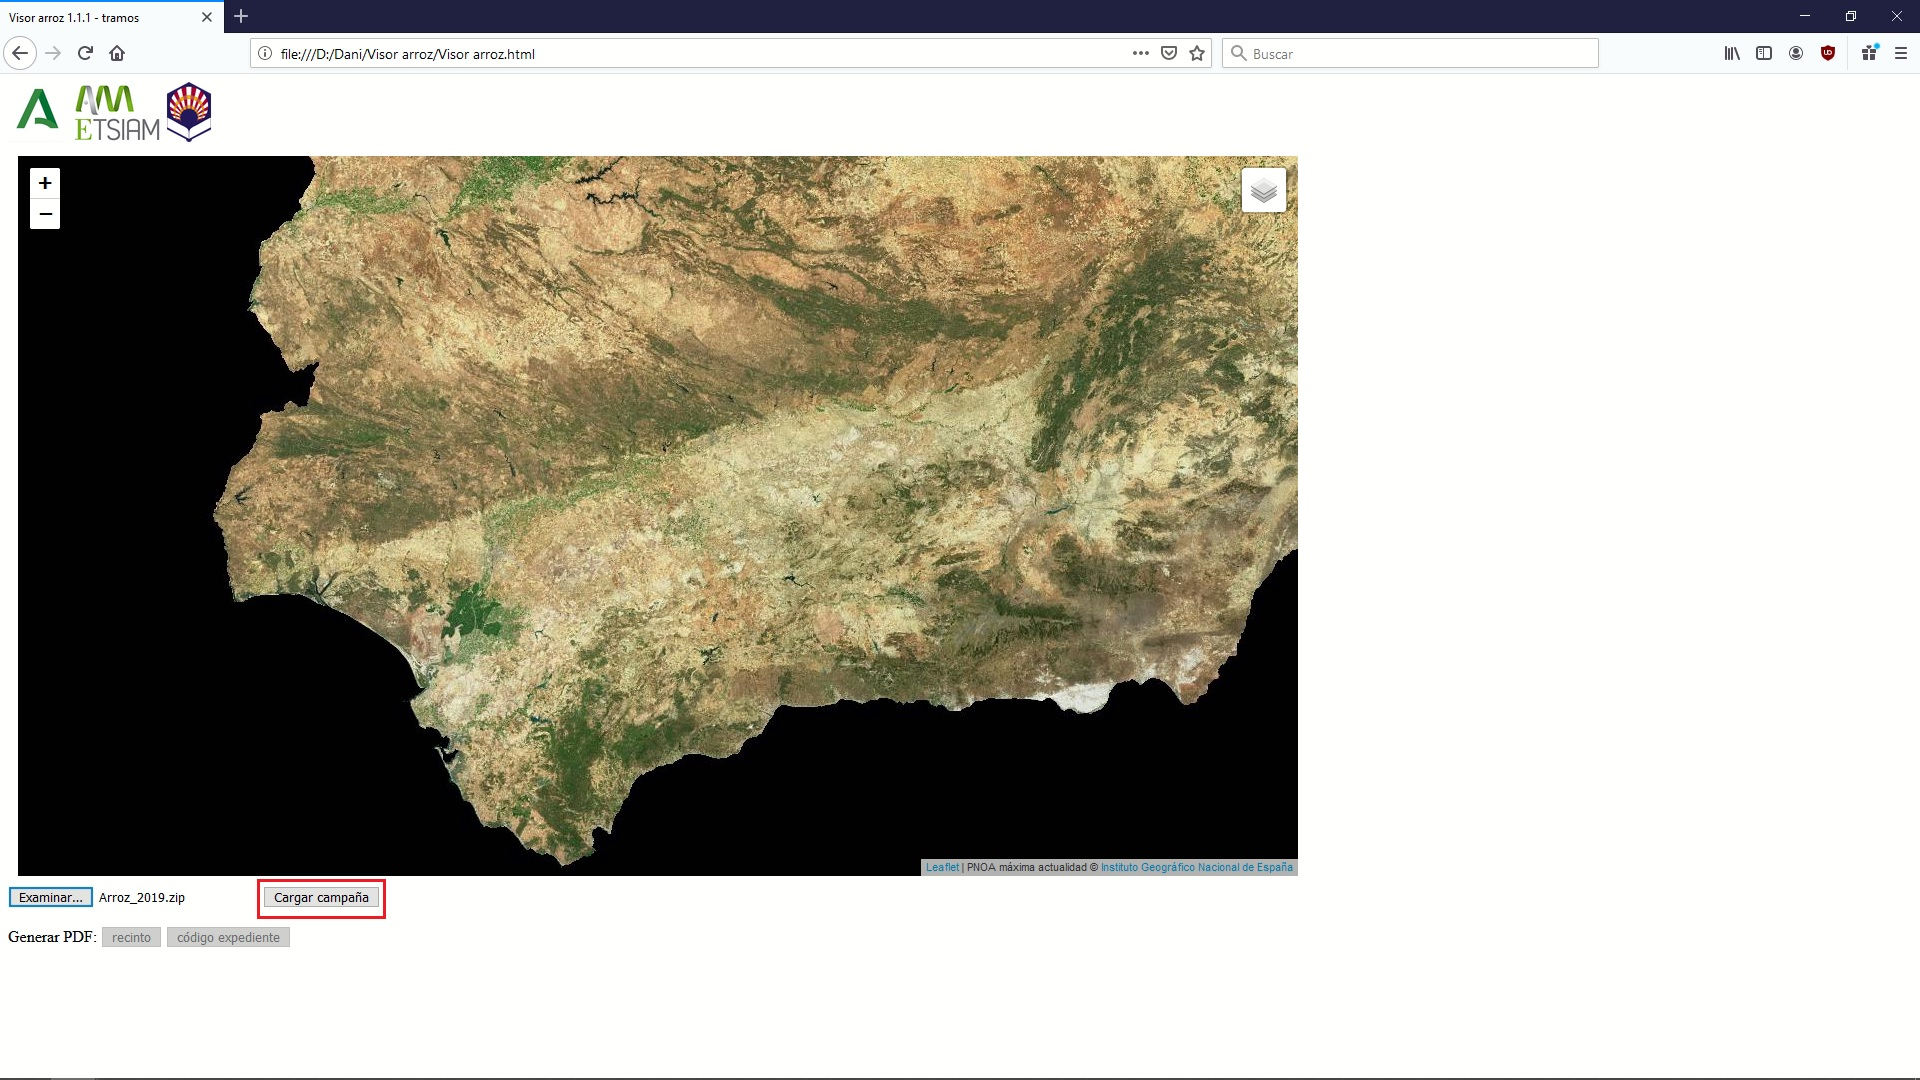
\includegraphics[width=0.8\linewidth]{cargar_campana.jpg}
	\caption{Cargando campaña}
	\label{fig:cargar_campana}
\end{figure}

Automáticamente comenzará la carga de dicha campaña en el visor, y se nos mostrará la geometría de los recintos en el mapa.

\begin{figure}[H]
	\centering
	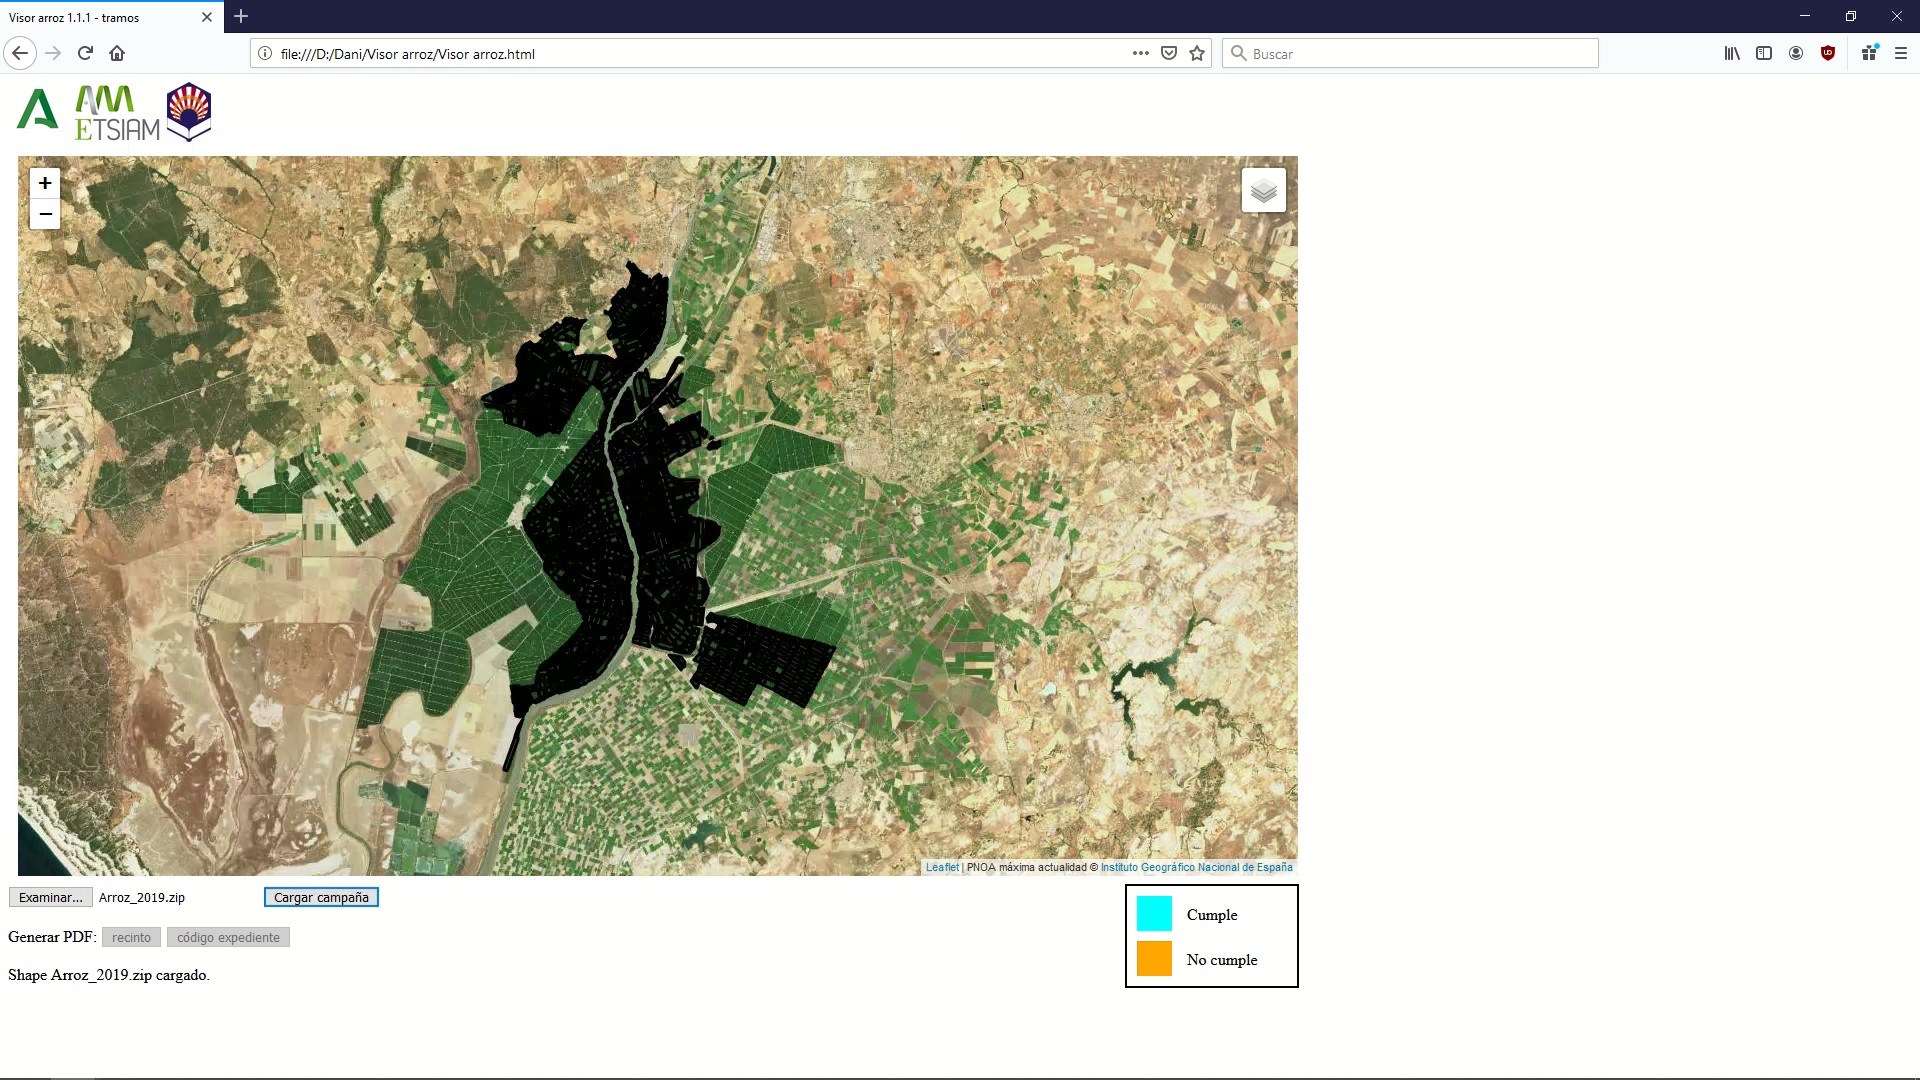
\includegraphics[width=0.8\linewidth]{campana_cargada.jpg}
	\caption{Campaña correctamente cargada}
	\label{fig:campana_cargada}
\end{figure}

\section{Seleccionar un recinto}

Para seleccionar un recinto, simplemente pinchamos en la geometría de un recinto que se quiera observar. Al hacerlo, se nos mostrarán las series temporales de los índices junto con la salida de la red coloreada por cada quincena, en la parte derecha del visor.

\begin{figure}[H]
	\centering
	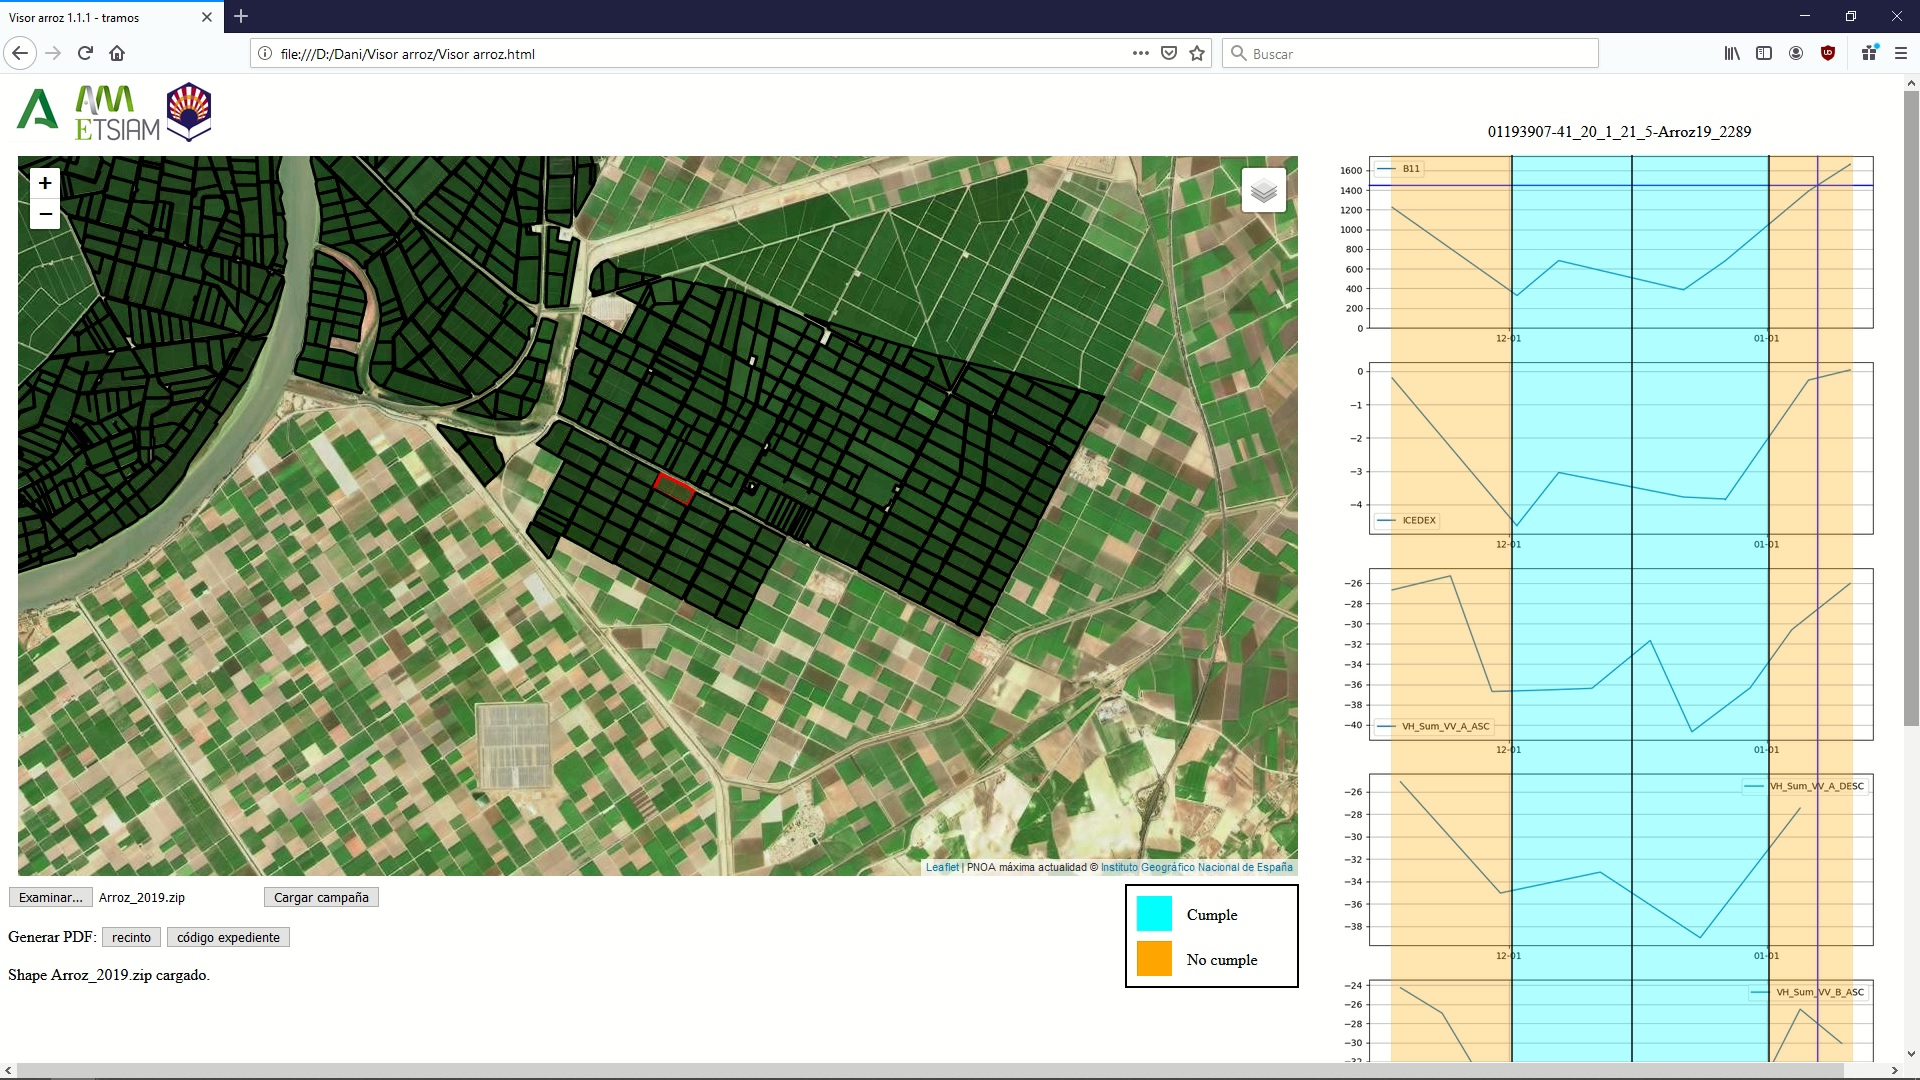
\includegraphics[width=0.8\linewidth]{recinto.jpg}
	\caption{Seleccionando un recinto}
	\label{fig:recinto}
\end{figure}

\section{Exportar un recinto}

Con esta opción, podemos exportar la información mostrada en el visor a un fichero .PDF. Para ello, debemos seleccionar primero un recinto, y posteriormente pinchar en el botón 'recinto'.

\begin{figure}[H]
	\centering
	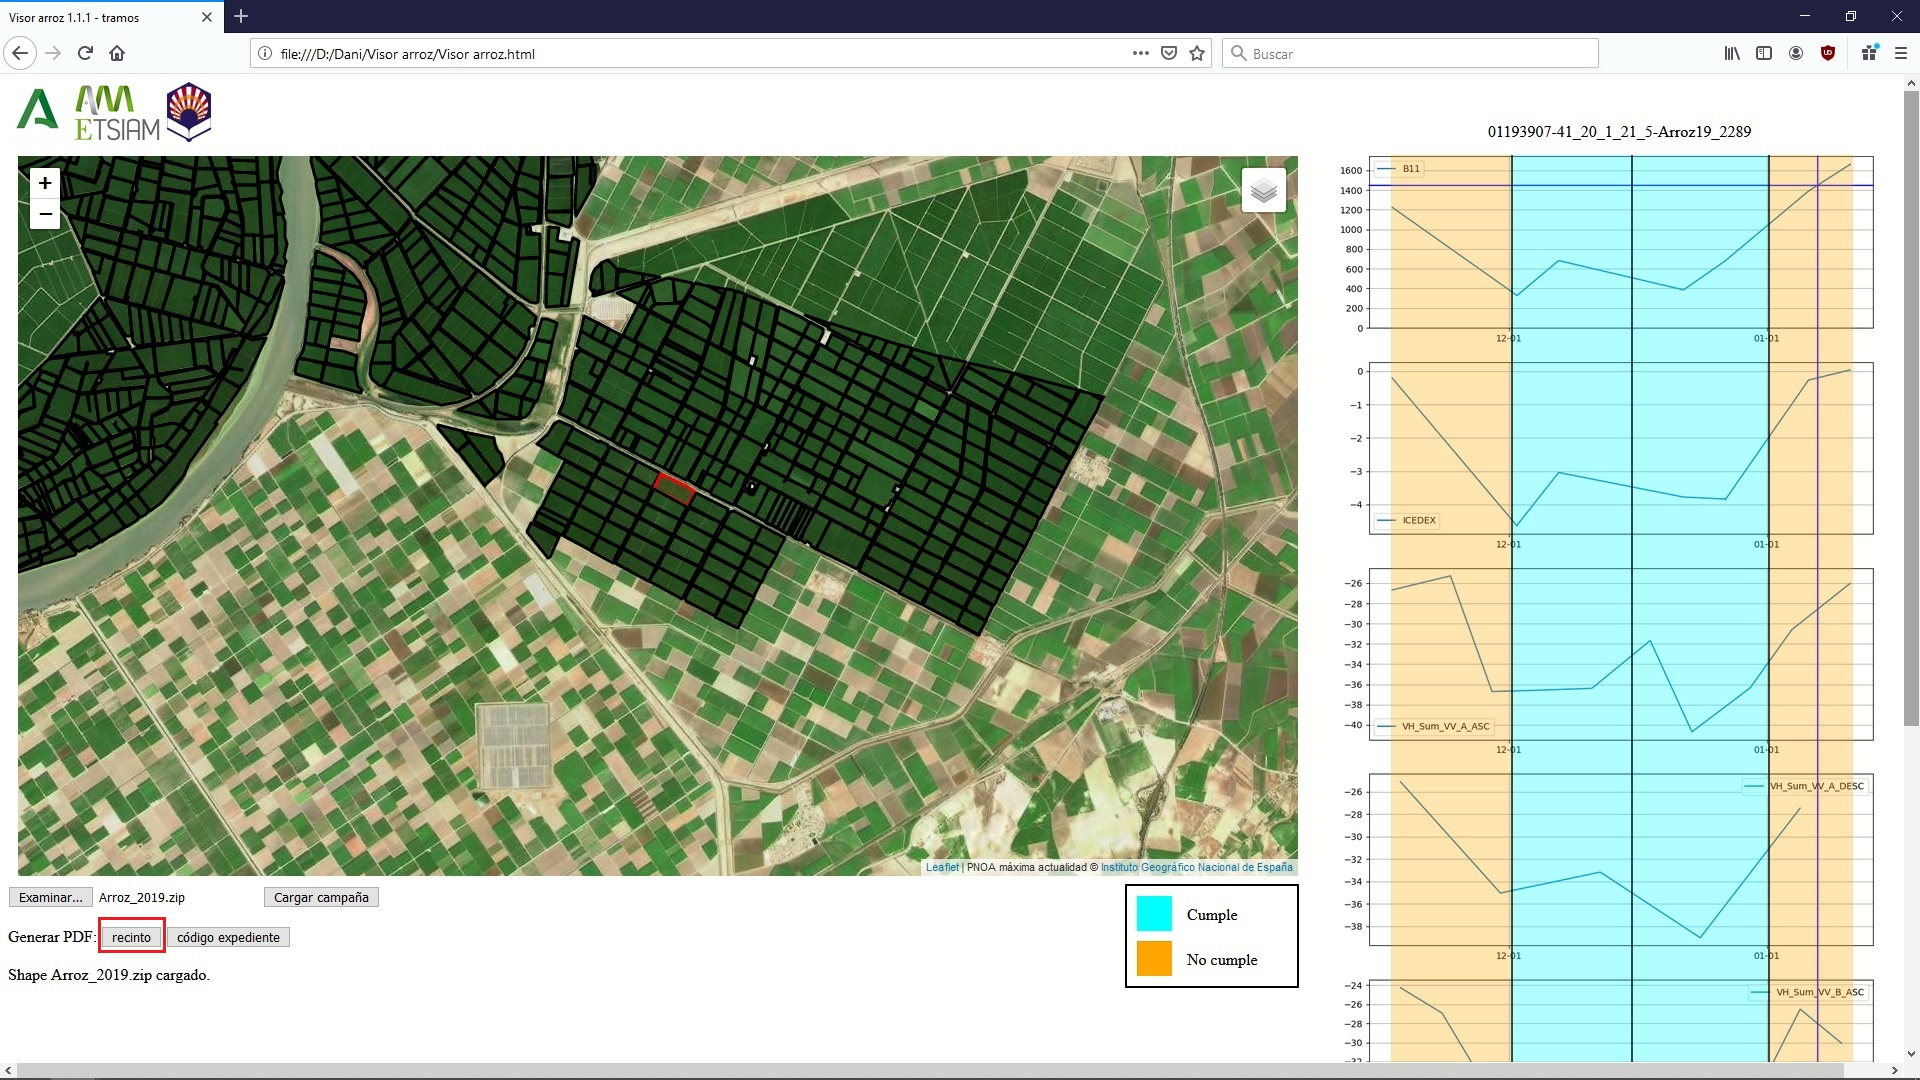
\includegraphics[width=0.8\linewidth]{guardar recinto.jpg}
	\caption{Guardando un recinto}
	\label{fig:guardar recinto}
\end{figure}

Se nos generará en la carpeta 'Descargas' un fichero 'PDF' con la información del visor.

\begin{figure}[H]
	\centering
	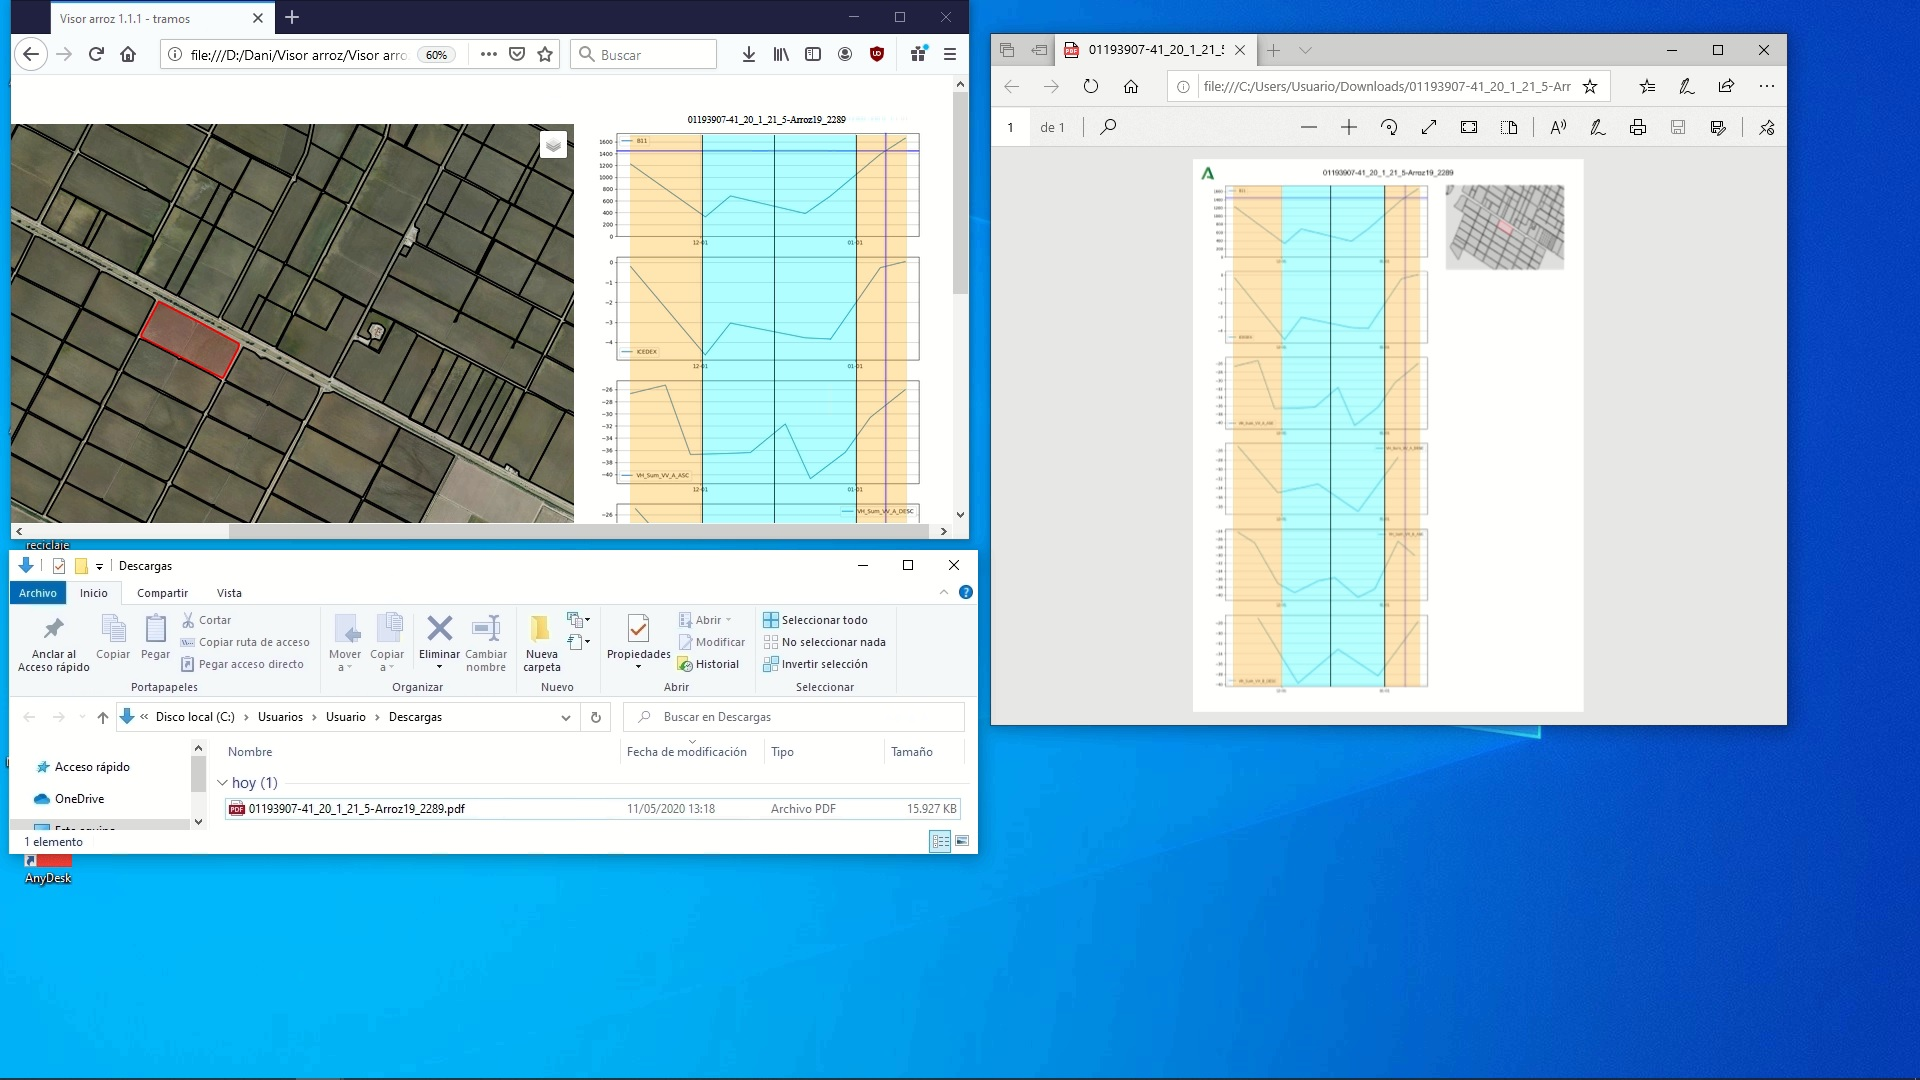
\includegraphics[width=0.8\linewidth]{pdf.jpg}
	\caption{Mostrando PDF}
	\label{fig:pdf}
\end{figure}

\section{Exportar recintos por código expediente}

Con esta opción se nos generará también ficheros PDFs, pero solo en aquellos recintos cuyo código expediente sea idéntico. Para ello, debemos primero seleccionar un recinto que tenga un número de expediente el cual queramos sacar todos los recintos que tengan en común dicho código. Posteriormente, una vez seleccionado el recinto deseado, pinchamos en el botón 'código expediente'

\begin{figure}[H]
	\centering
	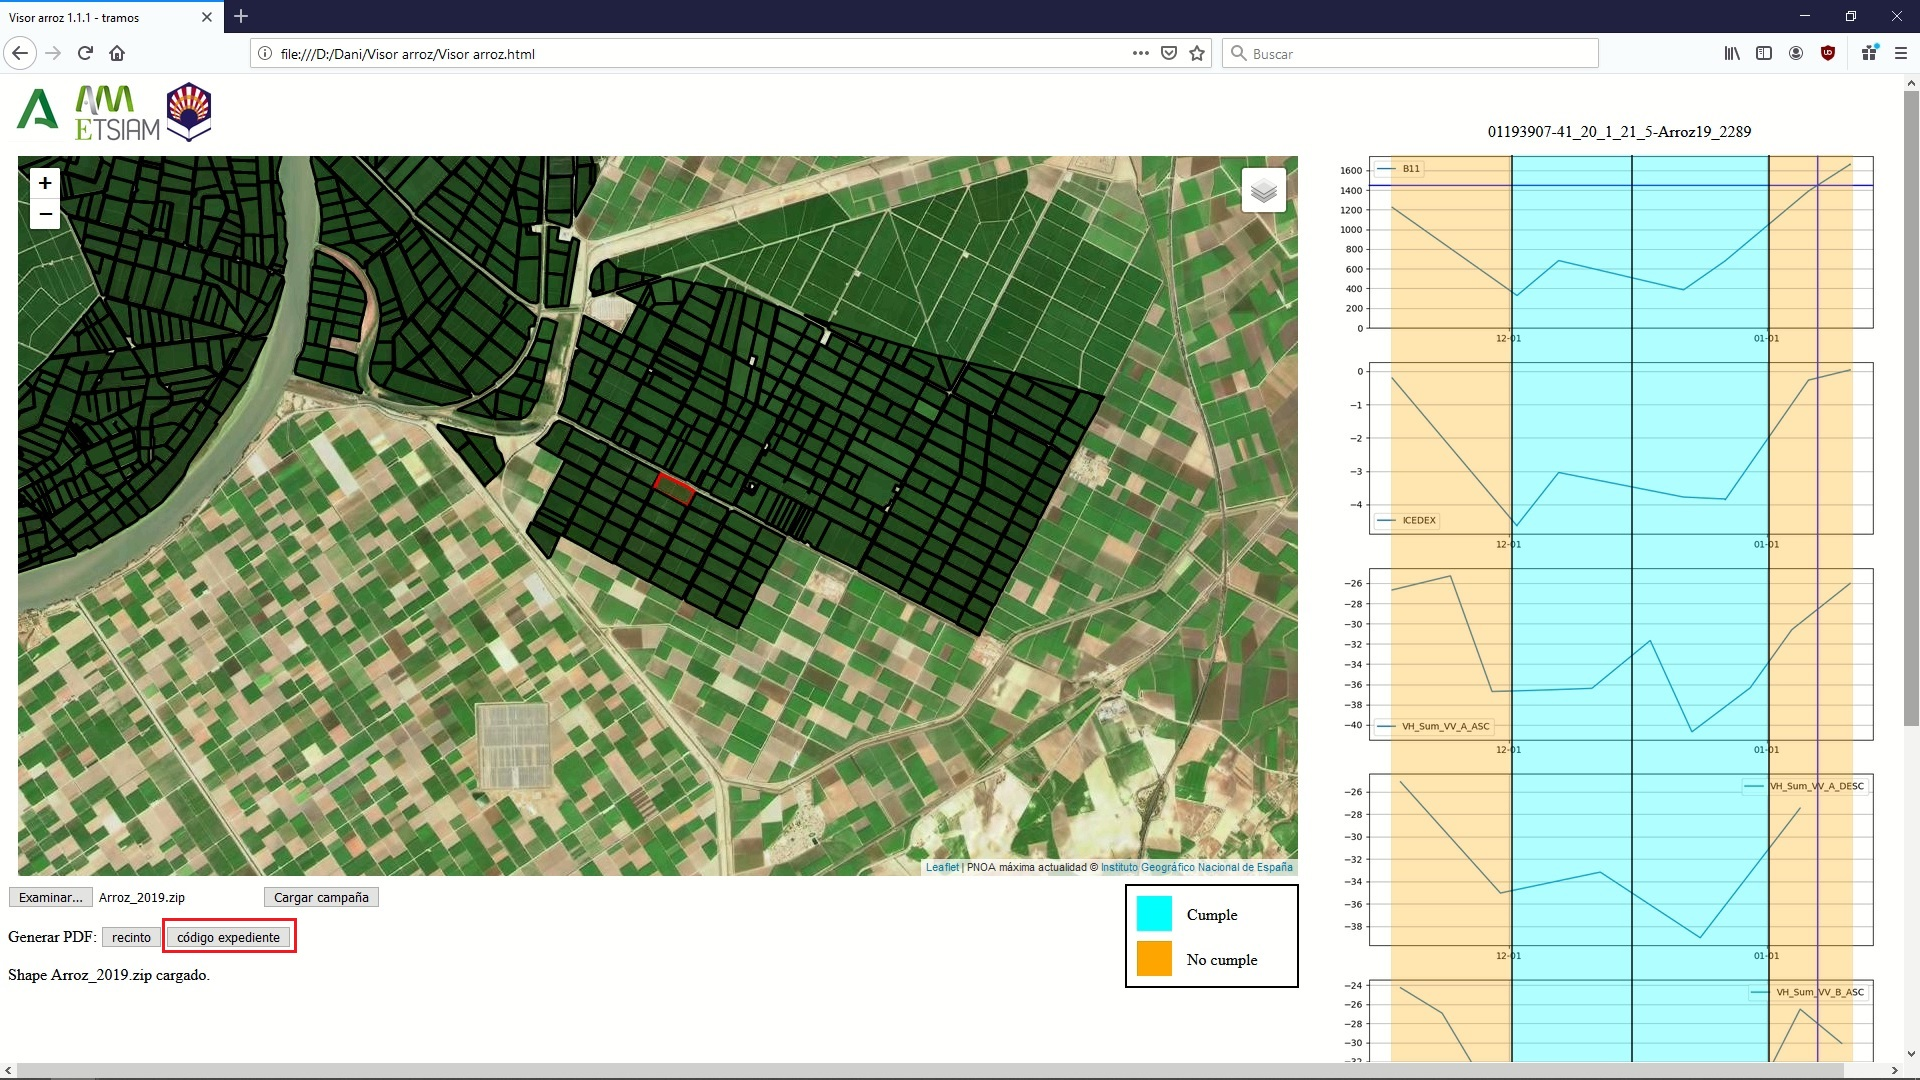
\includegraphics[width=0.8\linewidth]{codexp.jpg}
	\caption{Guardando varios PDFs por código expediente}
	\label{fig:codexp}
\end{figure}

Igual que en el caso anterior, tendremos en la carpeta 'Descargas', los diferentes PDFs de cada uno de los recintos con un mismo código de expediente.

\begin{figure}[H]
	\centering
	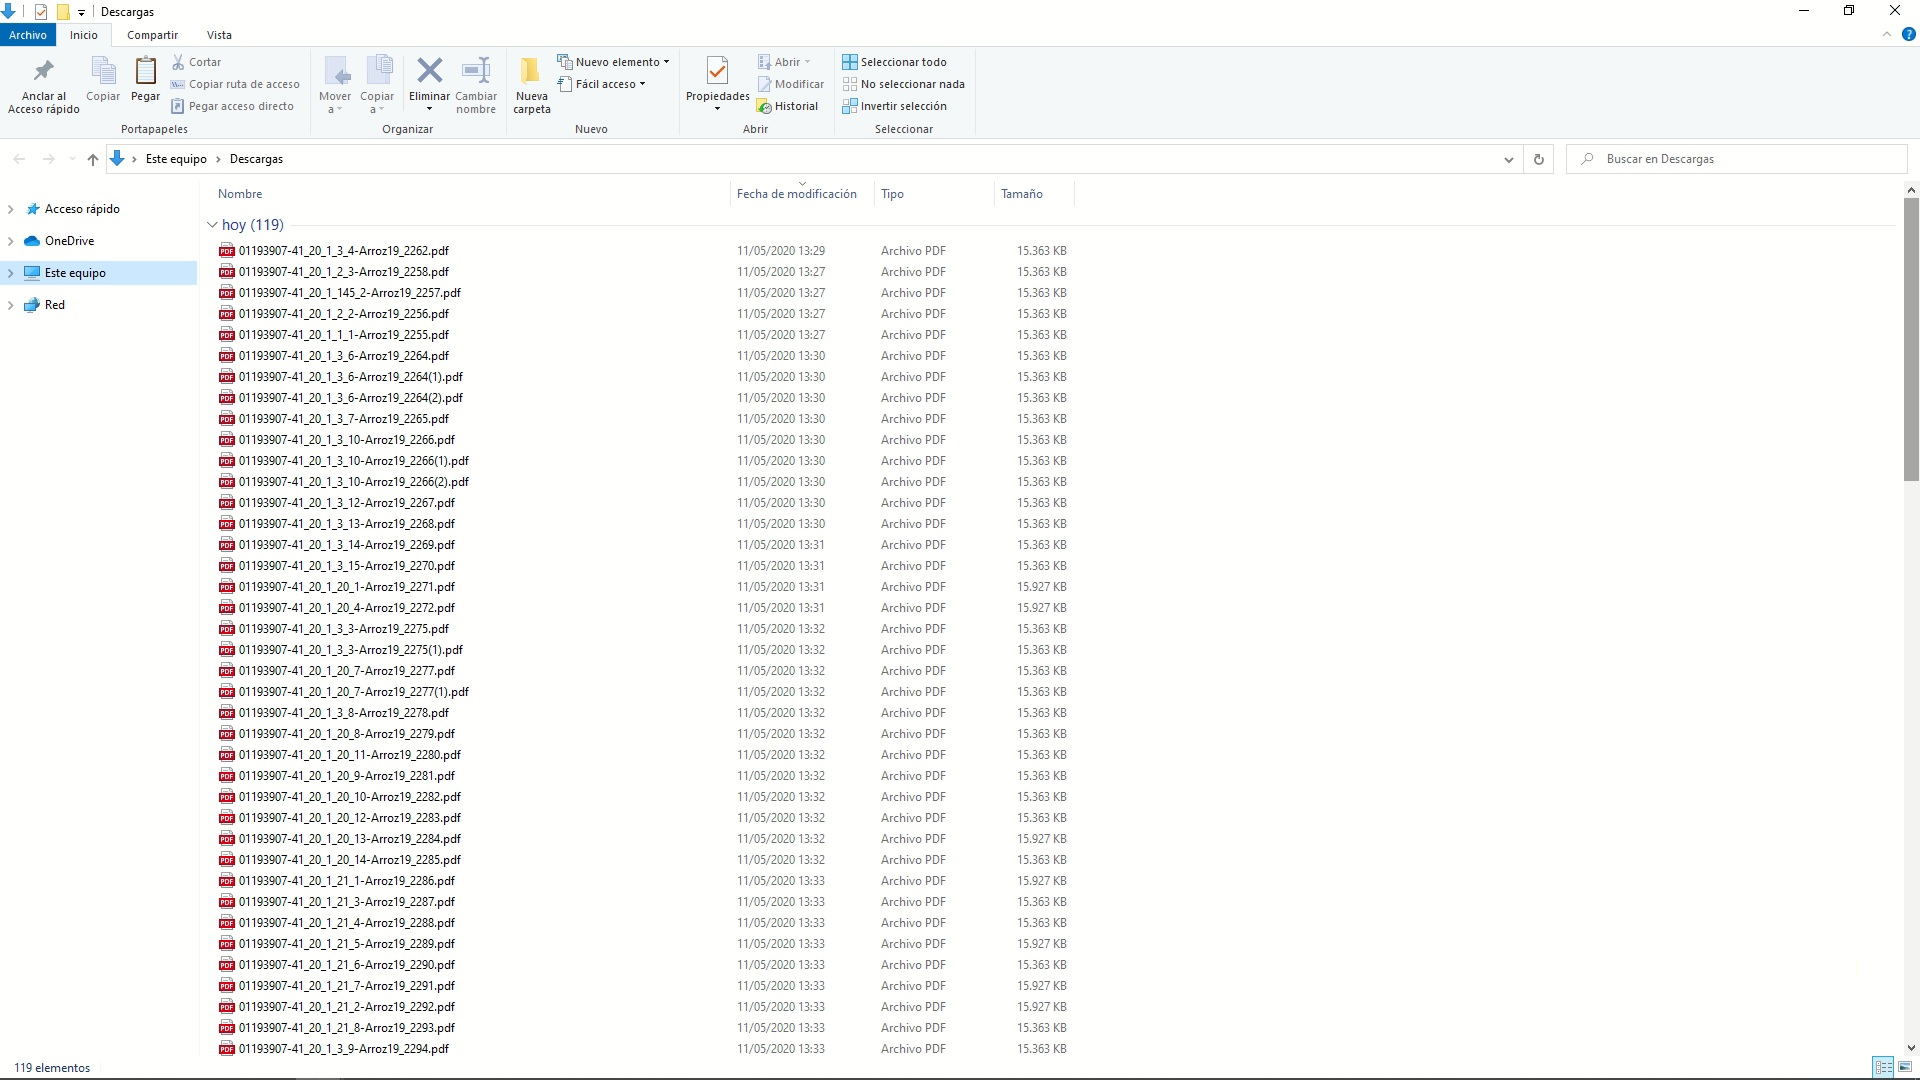
\includegraphics[width=0.8\linewidth]{pdfs.jpg}
	\caption{PDFs en la carpeta 'Descargas'}
	\label{fig:pdfs}
\end{figure}

\textbf{NOTA}: Al utilizar esta opción, en el navegador que utilice, le pedirá que las descargas de los ficheros PDFs se hagan automáticas, o bien le pedirá permisos. Es recomendable que le diga que sí, para que los PDFs se vayan descargando automáticamente.

\end{document}